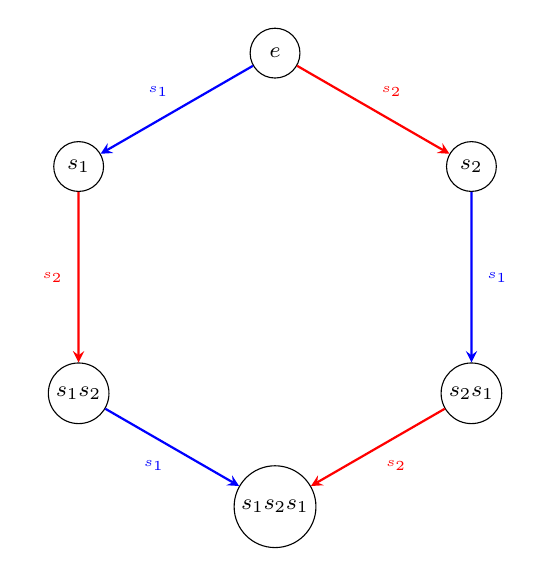
\begin{tikzpicture}[scale=1.6, every node/.style={circle, draw, fill=white, inner sep=2pt, minimum size=18pt, font=\footnotesize}]
    \node (e)   at (90:1.8)  {\(e\)};
    \node (s1)  at (150:1.8) {\(s_1\)};
    \node (s2)  at (30:1.8)  {\(s_2\)};
    \node (s1s2) at (210:1.8) {\(s_1 s_2\)};
    \node (s2s1) at (330:1.8) {\(s_2 s_1\)};
    \node (s1s2s1) at (270:1.8) {\(s_1 s_2 s_1\)};
    \draw[->, >=stealth, thick, blue] (e) -- node[draw=none, fill=none, above left, font=\tiny] {\(s_1\)} (s1);
    \draw[->, >=stealth, thick, red] (e) -- node[draw=none, fill=none, above right, font=\tiny] {\(s_2\)} (s2);
    \draw[->, >=stealth, thick, red] (s1) -- node[draw=none, fill=none, left, font=\tiny] {\(s_2\)} (s1s2);
    \draw[->, >=stealth, thick, blue] (s2) -- node[draw=none, fill=none, right, font=\tiny] {\(s_1\)} (s2s1);
    \draw[->, >=stealth, thick, blue] (s1s2) -- node[draw=none, fill=none, below left, font=\tiny] {\(s_1\)} (s1s2s1);
    \draw[->, >=stealth, thick, red] (s2s1) -- node[draw=none, fill=none, below right, font=\tiny] {\(s_2\)} (s1s2s1);
\end{tikzpicture}
